\section{Aproximación por Greedy}

Proponemos dos aproximaciones extra.

\subsubsection{Máximo por grupo}
Este enfoque realiza un cálculo de la frecuencia con la que cada jugador aparece en los $m$ subconjuntos $B$. Posteriormente, procede a recorrer cada uno de estos subconjuntos y, si la solución parcial propuesta no incluye ningún jugador presente en un subconjunto dado, se incluye en esta solución al jugador que tiene la mayor frecuencia de apariciones dentro de dicho subconjunto.

Este enfoque se distingue por su carácter greedy al enfocarse en optimizar la solución global mediante la búsqueda de óptimos locales en cada subconjunto. Se prioriza la inclusión del jugador con la mayor frecuencia de aparición en situaciones donde la solución parcial no incluye a ningún jugador del subconjunto evaluado. Este método busca mejorar la solución global al introducir jugadores de acuerdo con su frecuencia de aparición en los subconjuntos, minimizando así la cobertura de elementos dentro de la solución propuesta.

\lstinputlisting[language=Python, firstline=5, lastline=37]{../algoritmos/greedy.py}

La primera operación tiene complejidad $O(k \times m)$, con $k$ el promedio de jugadores por subconjunto ($k \leq n$). Con grupos más chicos, el algoritmo tiende a lineal ($O(m)$) y con grupos más grandes, a $O(m\times n)$. 
De la misma manera, la segunda operación tiene complejidad de  $O(m\times n)$ ya que por cada subconjunto ($O(k)$) se deben recorrer todos sus jugadores para verificar si efectivamente están en la solución final ($O(m)$) y, en caso de que no esté ninguno, se debe encontrar el jugador con máximas apariciones $O(m)$. Entonces, la complejidad total es $O(2(k \times m))=O(k \times m)$ y resulta polinomial.

\subsubsection{Máximo global con recálculo}

La segunda aproximación comienza de la misma manera, calculando la cantidad de apariciones de cada jugador en cada subconjunto. Luego agrega el jugador con más apariciones entre todos y quita las apariciones de los subconjuntos que ya cubre al resto de los jugadores. Realiza esta operación hasta quedarse sin jugadores restantes o que el jugador encontrado en la busqueda del de mayor frecuencia tenga cero apariciones restantes.

La ténica de diseño implementada en este algorítmo, al igual que el anterior explicado,  es greedy ya que busca el óptimo local al optimizar globalmente la solución por cada subconjunto, priorizando la inclusión del jugador con la mayor frecuencia hasta que se cumpla la cobertura de todos los conjuntos.

\lstinputlisting[language=Python, firstline=39, lastline=68]{../algoritmos/greedy.py}

Lla complejidad de la primera operación es $O(k \times m)$. La segunda tiene complejidad $O(j \times g \times m)$, con $j$ la cantidad de jugadores de la solución, $j \leq m$, y $g$ la cantidad promedio de grupos que cubre cada jugador $g \leq k$. Entonces, la complejidad total es $O(k \times m + j \times g \times m)$. %?

\section{Ejemplos}

A continuación, compararemos los resultados obtenidos por cada uno de los algoritmos con distintos ejemplos.

El primer ejemplo, ilustrado en la fig. \ref{fig:greedy_ej1}, es un caso feliz en el que los tres algoritmos obtienen el resultado óptimo.

\begin{figure}[H]
    \centering
    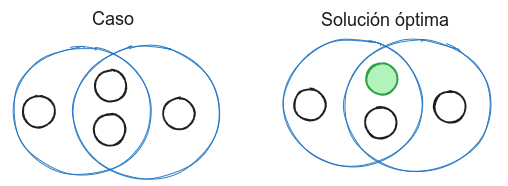
\includegraphics[width=0.8\textwidth]{img/greedy_ej1.png}
    \caption{Ejemplo 1}
    \label{fig:greedy_ej1}
\end{figure}

\begin{figure}[H]
    \centering
    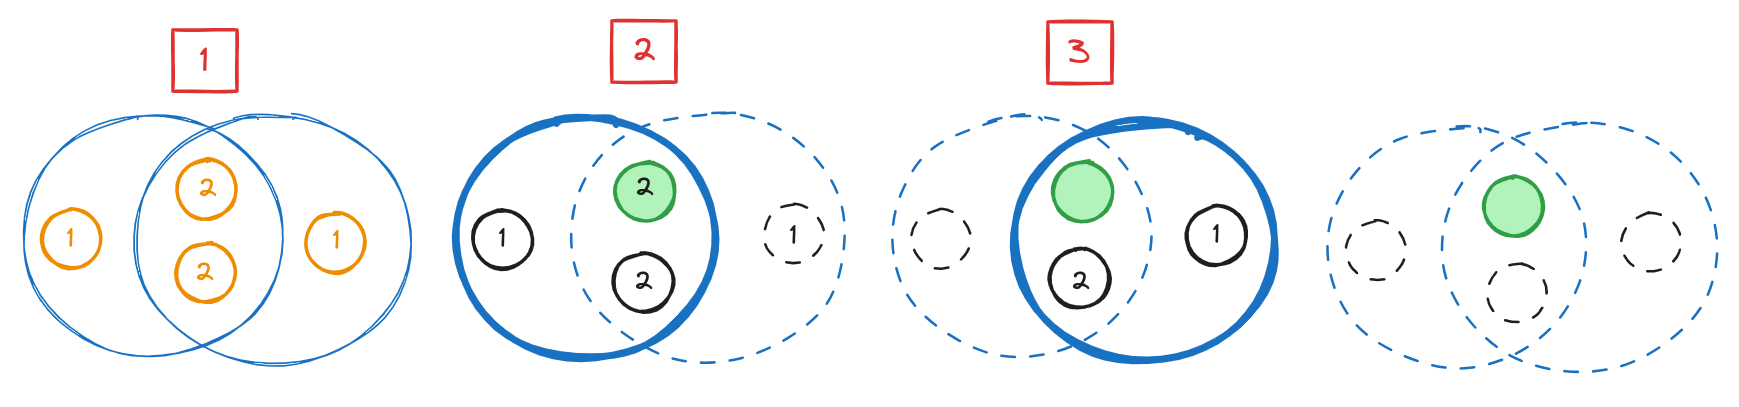
\includegraphics[width=0.8\textwidth]{img/greedy_ej1_mpg.png}
    \caption{Ejemplo 1 resuelto por Máximo por grupo}
    \label{fig:greedy_ej1_mpg}
\end{figure}

\begin{figure}[H]
    \centering
    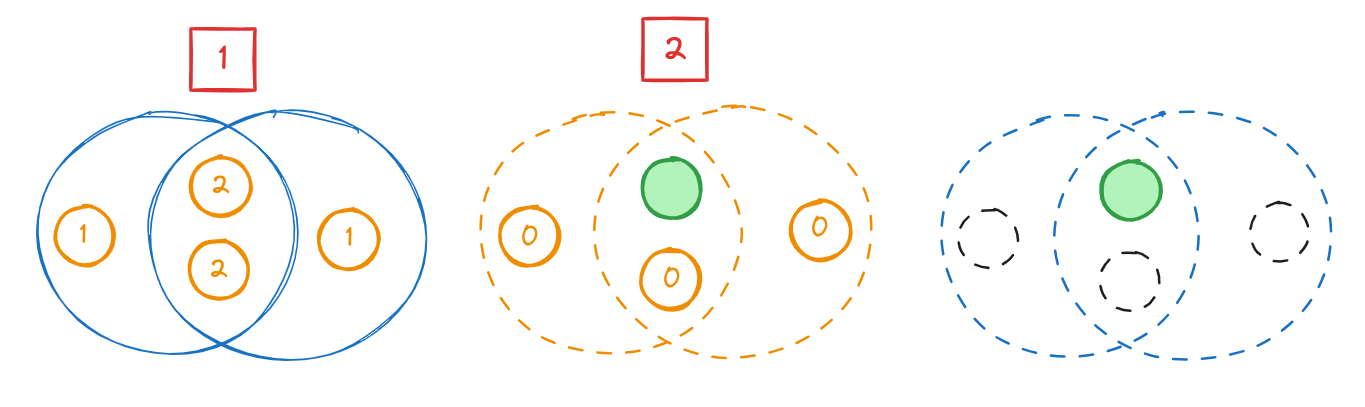
\includegraphics[width=0.8\textwidth]{img/greedy_ej1_mgr.png}
    \caption{Ejemplo 1 resuelto por Máximo global con recálculo}
    \label{fig:greedy_ej1_mgr}
\end{figure}

El segundo ejemplo (fig. \ref{fig:greedy_ej2}) podemos observar en la fig. \ref{fig:greedy_ej2_mpg} que "Máximo por grupo", de menor complejidad, no encuentra la solución óptima, pero el "Máximo global con recálculo", en la fig. \ref{fig:greedy_ej2_mgr}, si.

\begin{figure}[H]
    \centering
    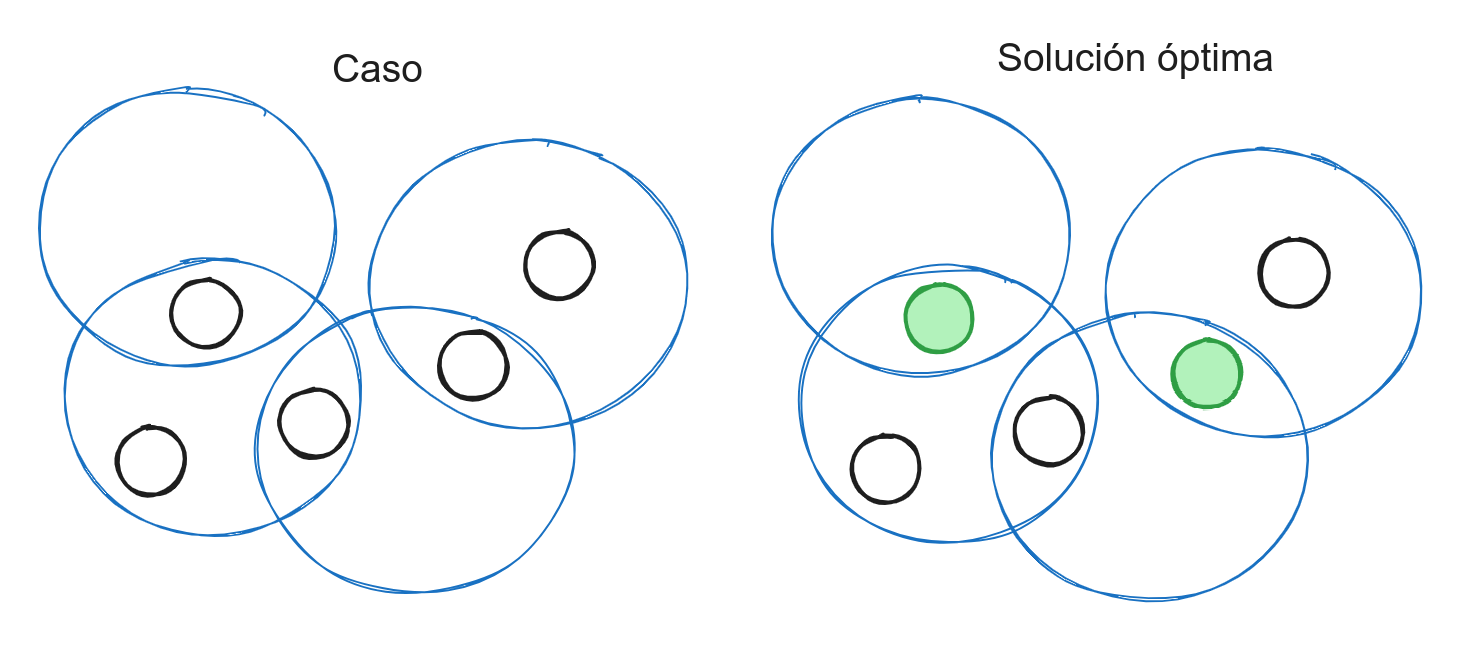
\includegraphics[width=0.8\textwidth]{img/greedy_ej2.png}
    \caption{Ejemplo 2}
    \label{fig:greedy_ej2}
\end{figure}

\begin{figure}[H]
    \centering
    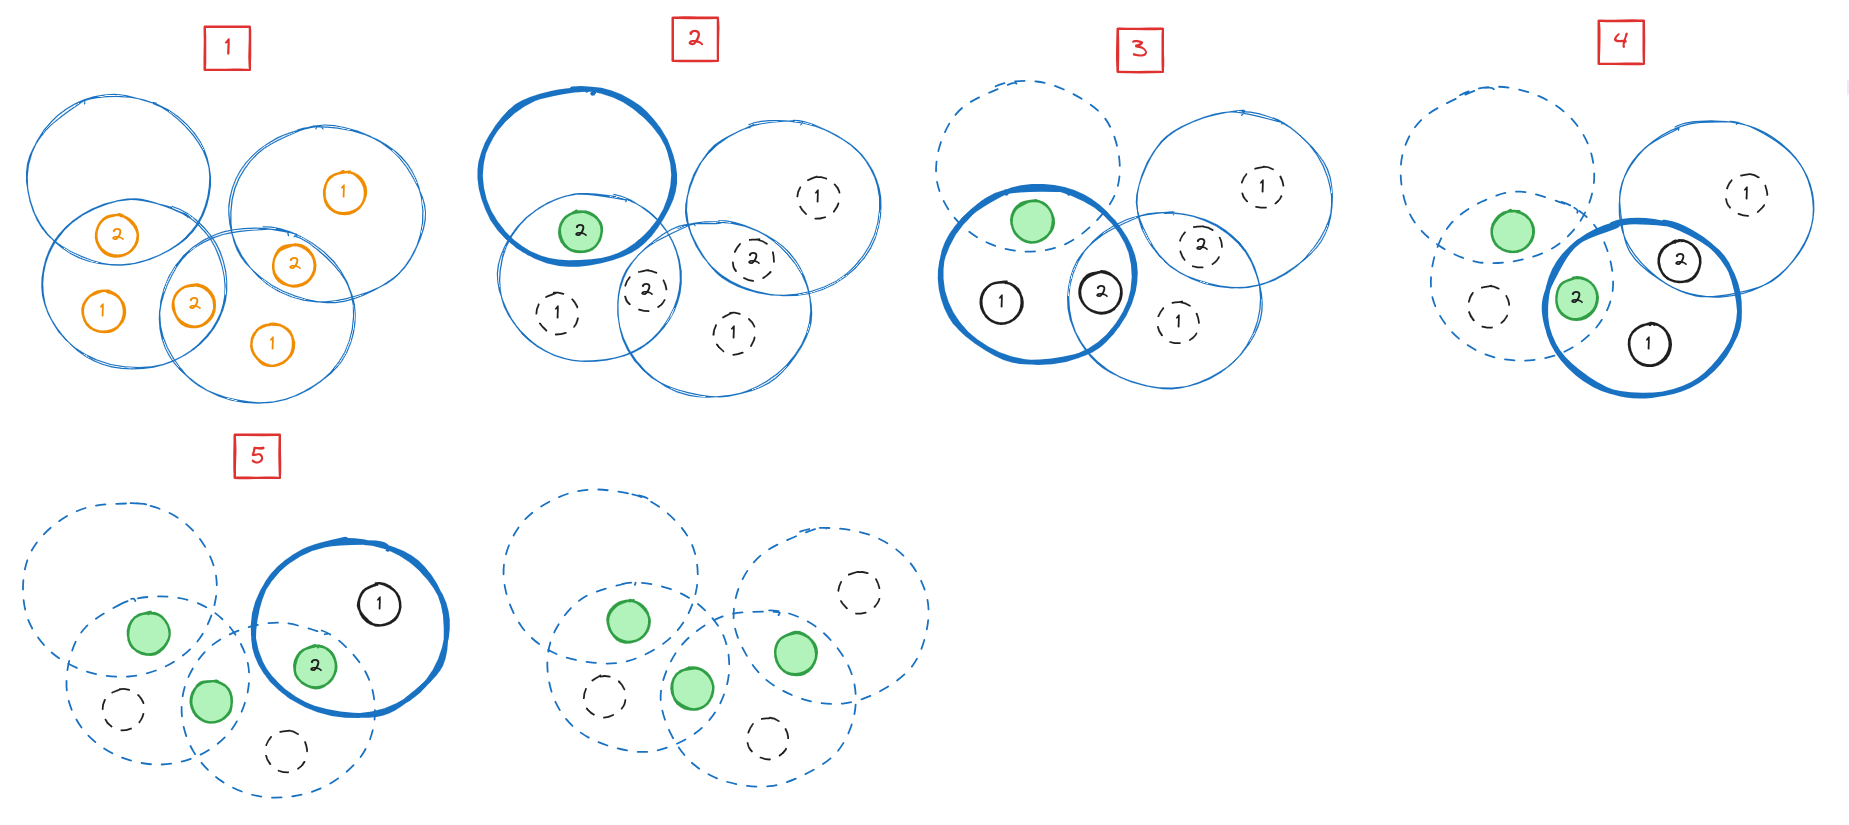
\includegraphics[width=0.8\textwidth]{img/greedy_ej2_mpg.png}
    \caption{Ejemplo 2 resuelto por Máximo por grupo}
    \label{fig:greedy_ej2_mpg}
\end{figure}

\begin{figure}[H]
    \centering
    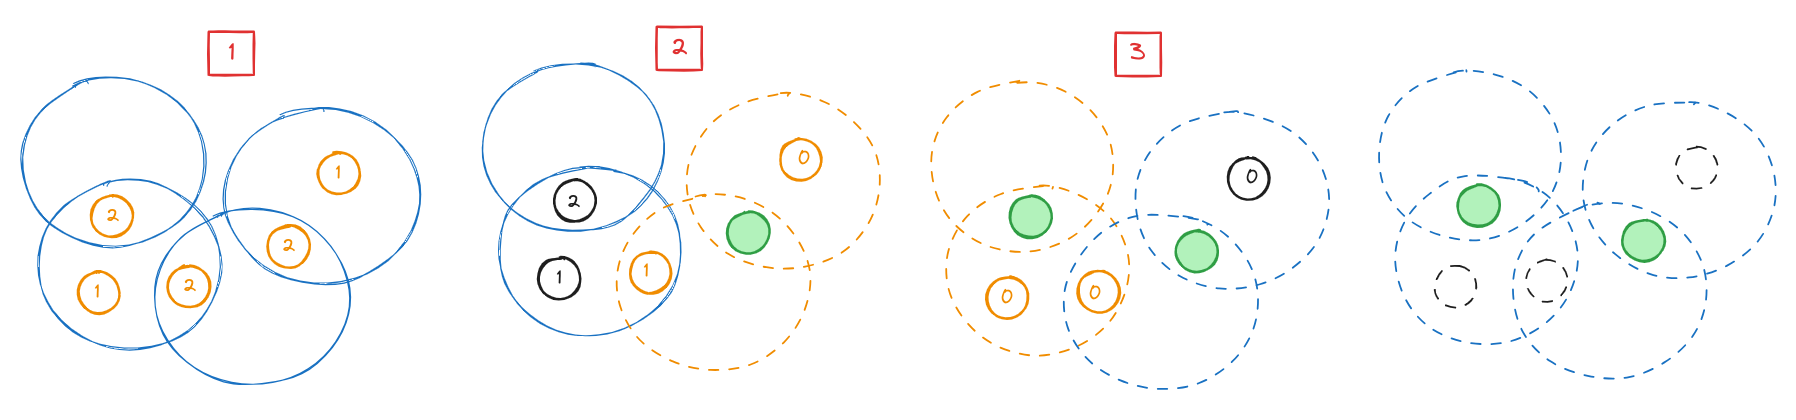
\includegraphics[width=0.8\textwidth]{img/greedy_ej2_mgr.png}
    \caption{Ejemplo 2 resuelto por Máximo global con recálculo}
    \label{fig:greedy_ej2_mgr}
\end{figure}

Por último, en el ejemplo de la fig. \ref{fig:greedy_ej3}, tanto "Máximo por grupo" (fig. \ref{fig:greedy_ej3_mpg}) como "Máximo global con recálculo" (fig. \ref{fig:greedy_ej3_mgr}) no llegan al la solución óptima.

\begin{figure}[H]
    \centering
    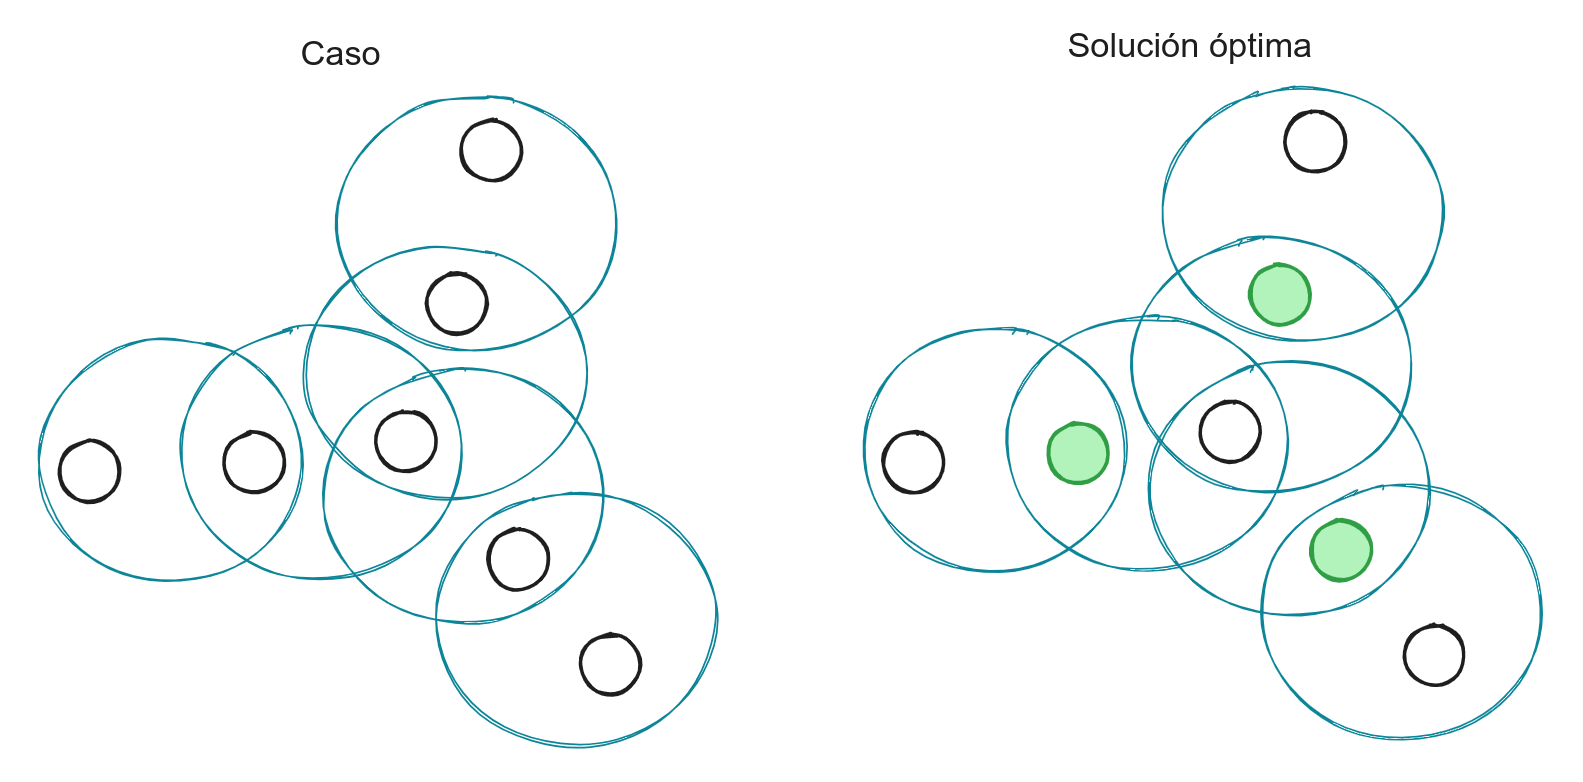
\includegraphics[width=0.8\textwidth]{img/greedy_ej3.png}
    \caption{Ejemplo 3}
    \label{fig:greedy_ej3}
\end{figure}

\begin{figure}[H]
    \centering
    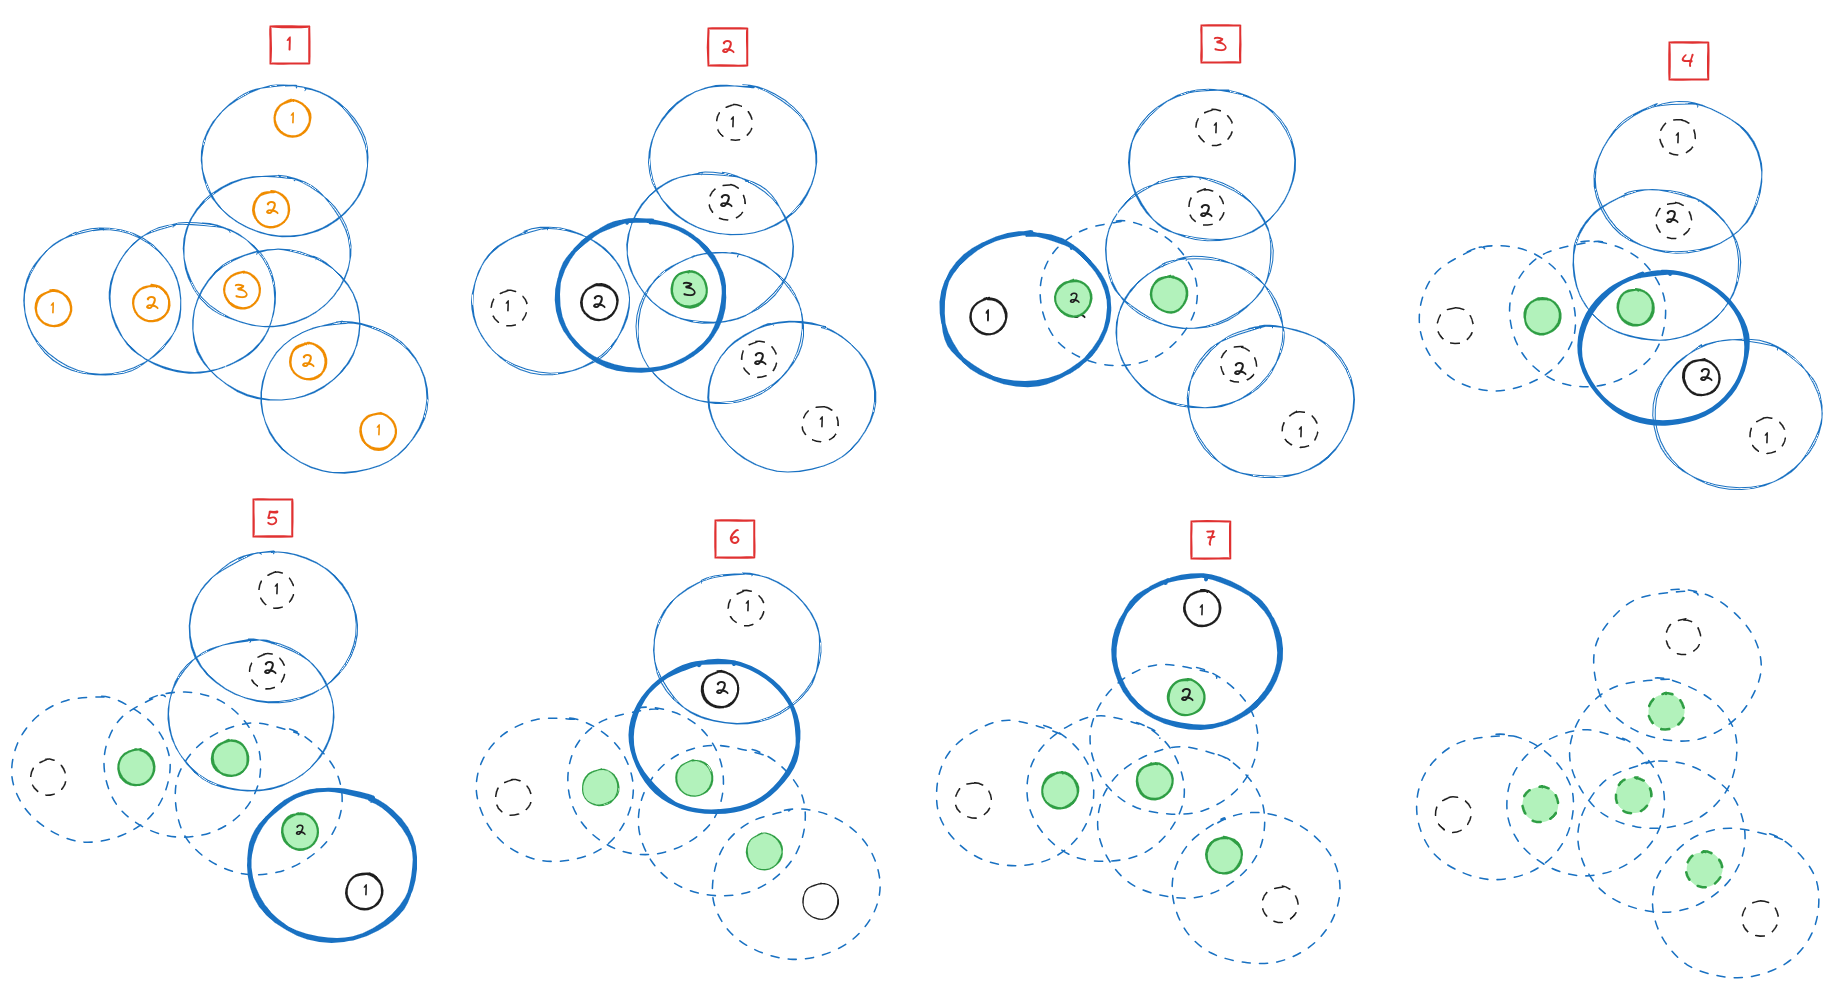
\includegraphics[width=0.8\textwidth]{img/greedy_ej3_mpg.png}
    \caption{Ejemplo 3 resuelto por Máximo por grupo}
    \label{fig:greedy_ej3_mpg}
\end{figure}

\begin{figure}[H]
    \centering
    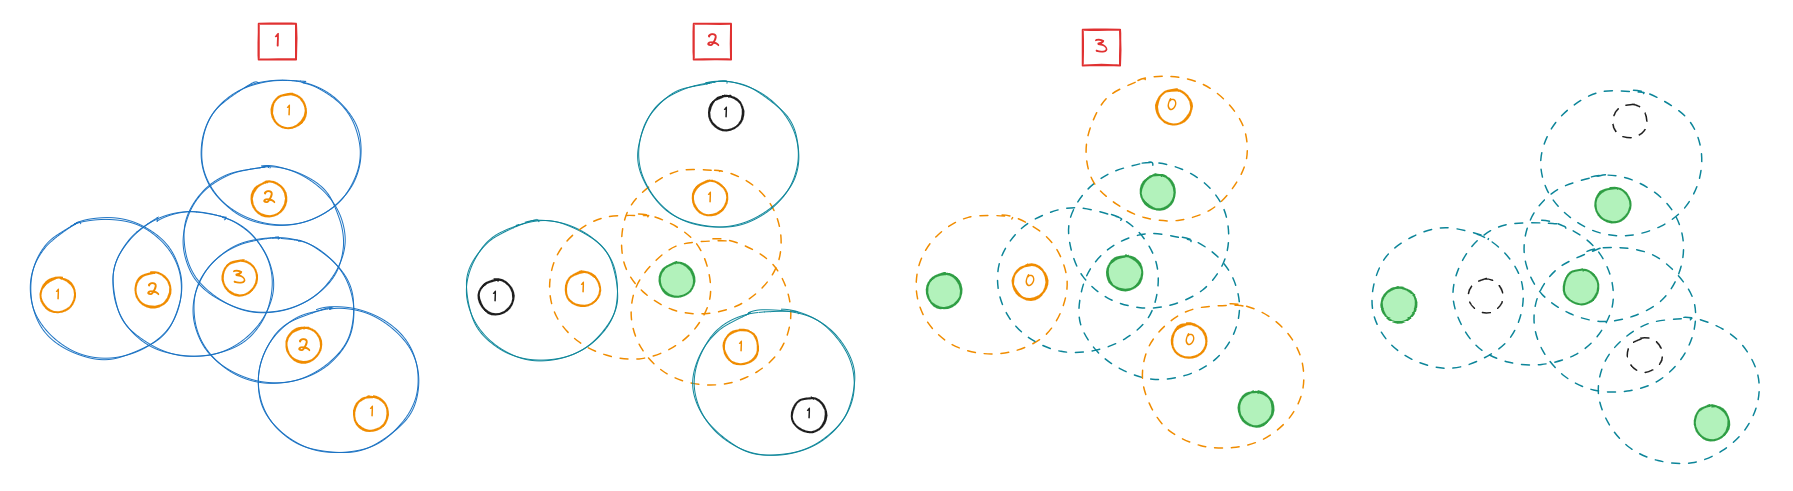
\includegraphics[width=0.8\textwidth]{img/greedy_ej3_mgr.png}
    \caption{Ejemplo 3 resuelto por Máximo global con recálculo}
    \label{fig:greedy_ej3_mgr}
\end{figure}